\documentclass[10pt]{article}
\usepackage[utf8]{inputenc}
\usepackage{mathtools}
\usepackage{amsmath}
\usepackage{graphicx}
\usepackage{array}
\usepackage[margin=0.5in]{geometry}
\usepackage{listings}
\usepackage{color}

\definecolor{mygreen}{rgb}{0,0.6,0}
\definecolor{mygray}{rgb}{0.5,0.5,0.5}
\definecolor{mymauve}{rgb}{0.58,0,0.82}

\lstset{ %
  backgroundcolor=\color{white},   % choose the background color; you must add \usepackage{color} or \usepackage{xcolor}; should come as last argument
  basicstyle=\footnotesize,        % the size of the fonts that are used for the code
  breakatwhitespace=false,         % sets if automatic breaks should only happen at whitespace
  breaklines=true,                 % sets automatic line breaking
  captionpos=b,                    % sets the caption-position to bottom
  commentstyle=\color{mygreen},    % comment style
  deletekeywords={...},            % if you want to delete keywords from the given language
  escapeinside={\%*}{*)},          % if you want to add LaTeX within your code
  extendedchars=true,              % lets you use non-ASCII characters; for 8-bits encodings only, does not work with UTF-8
  frame=single,	                   % adds a frame around the code
  keepspaces=true,                 % keeps spaces in text, useful for keeping indentation of code (possibly needs columns=flexible)
  keywordstyle=\color{blue},       % keyword style
  language=Octave,                 % the language of the code
  morekeywords={*,...},            % if you want to add more keywords to the set
  numbers=left,                    % where to put the line-numbers; possible values are (none, left, right)
  numbersep=5pt,                   % how far the line-numbers are from the code
  numberstyle=\tiny\color{mygray}, % the style that is used for the line-numbers
  rulecolor=\color{black},         % if not set, the frame-color may be changed on line-breaks within not-black text (e.g. comments (green here))
  showspaces=false,                % show spaces everywhere adding particular underscores; it overrides 'showstringspaces'
  showstringspaces=false,          % underline spaces within strings only
  showtabs=false,                  % show tabs within strings adding particular underscores
  stepnumber=2,                    % the step between two line-numbers. If it's 1, each line will be numbered
  stringstyle=\color{mymauve},     % string literal style
  tabsize=2,	                   % sets default tabsize to 2 spaces
  title=\lstname                   % show the filename of files included with \lstinputlisting; also try caption instead of title
}
\renewcommand{\arraystretch}{1.5}
\setcounter{secnumdepth}{0}
\author{Kevin Mambu}
\date{\today}
\title{M1 SESI 2017-2018\\Architecture Multi-Processeurs\\TP4 : Partage du Bus
dans les architectures multi-processeurs}

\begin{document}
\maketitle
\section{Spécifications}
Objectifs :
\begin{itemize}
  \item Problèmes de performances posés par le partage du bus.
  \item Goulot d'étranglement lorsque plusieurs processeurs veulent accéder au
  bus car \underline{la bande passante du bus est bornée}.
  \item Temps d'attente du bus proportionnel au nombre de processeurs dans
  l'architecture.
\end{itemize}

\section{B) Architecture Matérielle}
\begin{itemize}
  \item Chaque processeur a un TTY attribué\\
  $\rightarrow$ N TTYs pour un contrôleur de TTY.
  \item $|seg\_tty| = {NPROC}\times{16}$.
  Utilisation d'un framebuffer $({256}\times{256})$ sur 256 niveaux de gris.
  \item Spécifications du framebuffer
  \begin{itemize}
    \item Un tampon de luminence, 64Ko
    \item Un tampon de chrominance, 64Ko, pas utilisé ici
    \item Fréquence de la lecture des tampons : 25 images par seconde
    \item Fréquence d'affichage : $f=\frac{1}{{40}\times{10^-3}}={250}Hz$
  \end{itemize}
\end{itemize}

\subsection{Question B1}
\begin{itemize}
  \item name : nom de l'instance
  \item tgtid : index du signal du framebuffer vis-à-vis du PIBUS
  \item segtab : pointeur vers la table des segments
  \item latency : temps d'accès au framebuffer
  \item width : largeur de l'image (en pixels)
  \item height : hauteur de l'image (en pixels)
  \item subsampling : fréquence de sous'échantillonage de la chrominance
  (ici non-utilisé)
\end{itemize}

\subsection{Question B2}
Le segment associé au Framebuffer doit être aligné et sa taille doit être de
${width}\times{height}$ octets (ici ${256}\times{256}=64$Ko).

\subsection{Dimensionnement des caches}
\begin{itemize}
  \item Caches Write-Through
  \item Correspondance directe
  \item 16 lignes de 8 mots
  \lstinputlisting[firstnumber=29,linerange={29-43},language={C++}]{tp5_top.cpp}
\end{itemize}

\section{C) Compilation de l'application logicielle}
\subsection{Question C1}
Le segment associé au contrôleur du Framebuffer fait partie de l'espace
privilégié. Tout accès mémoire de l'application utilisateur avec le Framebuffer
doit passer par un appel système pour être légal. À cause d'un manque de
permissions de la part de l'application utilisateur, un accès direct avec le
Framebuffer se traduirait par un Data Bus Error.

\subsection{Question C2}
Écrire ligne par ligne limite le nombre de transactions sur le PIBUS à une seule
transaction rafale, une fois le registre intermédiaire plein. Plutôt qu'une
transaction par octet, ce qui est plus coûteux.

\subsection{Question C3}
{\it unsigned int fb\_sync\_write(unsigned int offset, void *buffer,unsigned int length)}
\begin{itemize}
  \item offset : le déplacement nécessaire où écrire dans le tampon du
  Framebuffer.\\
  *note : sachant qu'on écrit sur le Framebuffer ligne par ligne, l'offset doit
  être aligné (multiple de 256).
  \item buffer : addresse de base du tampon intermédiaire
  \item : longeur en octets de la donnée à écrire sur le framebuffer.
\end{itemize}

\newpage

\section{D) Caractérisation de l'application logicielle}
\subsection{Question D1}
Execution à un processeur :
\begin{center}
  \begin{tabular}{|c|c|c|}
    \hline
    \texttt{NB\_CYCLES} & \texttt{NB\_INST} & \texttt{CPI} \\ \hline
    $5697418$ & $4010805$ & $1.42052$ \\ \hline
  \end{tabular}
\end{center}

\subsection{Question D2}
\begin{center}
  \begin{tabular}{|c|c|c|c|}
    \hline
    \texttt{WRITE\_RATE} & \texttt{READ\_RATE} & \texttt{IMISS\_RATE} & \texttt{DMISS\_RATE} \\ \hline
    $0.142853$ & $0.267784$ & $0.008941$ & $0.009121$ \\ \hline
    \texttt{IMISS\_COST} & \texttt{DMISS\_COST} & \texttt{WRITE\_COST} & \\ \hline
    $16.0537$ & $14.3444$ & $0.0000$ & \\ \hline
  \end{tabular}
\end{center}
Les coûts sont des valeurs non-entières parce qu'elles sont moyennées.

\subsection{Question D3}
Nombres de transacations :
\begin{center}
  \begin{tabular}{|c|c|c|c|}
    \hline
    \texttt{IMISS} & \texttt{DMISS} & \texttt{UNC} & \texttt{WRITE} \\ \hline
    $35860$ & $36582$ & $5266$ & $572955$ \\ \hline
  \end{tabular}
\end{center}
Si le nombre de transactions de lectures est relativement faible, le nombre de
transactions d'écritures lui est bien plus conséquent. Cela doit être dû au
fait que les écritures sont prioritaires.

\section{E) Exécution sur architecture multi-processeur}
\subsection{Question E1}
\lstinputlisting[language=C,linerange={20-43}]{main.c}

\newpage

\subsection{Question E2}
\lstinputlisting{reset.s}

\subsection{Question E3}
Le fichier config.h spécifie la constante \texttt{NB\_PROC}, le nombre de
processeurs. De ce fait, à chaque fois que l'on modifie le nombre de processeurs
il faut re-génerer le binaire du programme.
\newpage

\subsection{Question E4}
\begin{center}
  \lstinputlisting[language=Gnuplot]{QuestionE4.plot}
  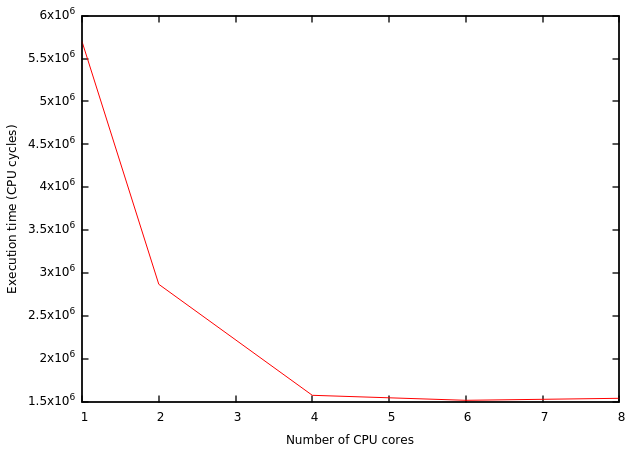
\includegraphics[width=8.5cm]{QuestionE4_1.png}
  \quad\quad
  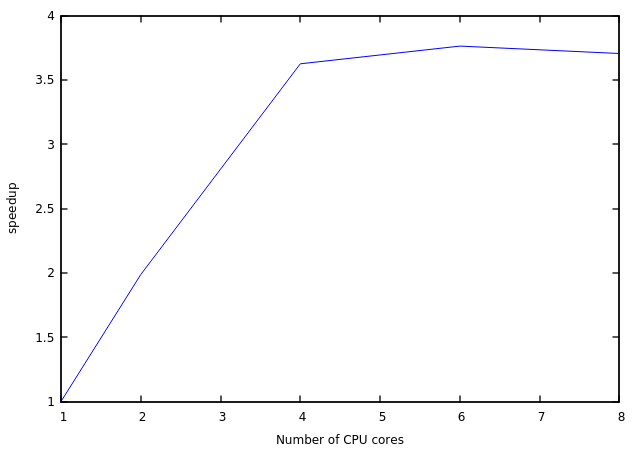
\includegraphics[width=8.5cm]{QuestionE4_2.png}
\end{center}

Posons l'équation suivante :
\begin{equation}
  \begin{split}
    speedup & =\frac{execution\_time(1)}{execution\_time(N)} \\
     & =\frac{execution\_time(1)}{N \times execution\_time(\frac{1}{N})}
  \end{split}
\end{equation}
Théoriquement, plus le nombre de processeurs augmente, plus le temps d'execution
par CPU diminue en fonction du nombre de processeurs, car ces derniers se partagent
la charge de l'exécution d'instructions et par extension du nombre de MISS.\\
Mais cette formule ne prend pas en compte la bande passante maximale du BUS, et
on peut le constater sur l'évolution des courbes ci-dessus : à partir de 4 coeurs,
le speedup ralentit considérablement et passé 6 coeurs le speedup diminue. Parce
que le bus est devenu un goulôt d'étranglement.

\newpage

\subsection{Question F1}
Au delà de l'exécution du programme, d'autres instructions continuent à être
exécutées et les comptabiliser fausserait notre instrumentation.

\subsection{Quesion F2}
\begin{center}
  \lstinputlisting[language=Gnuplot]{QuestionF2.dat}
  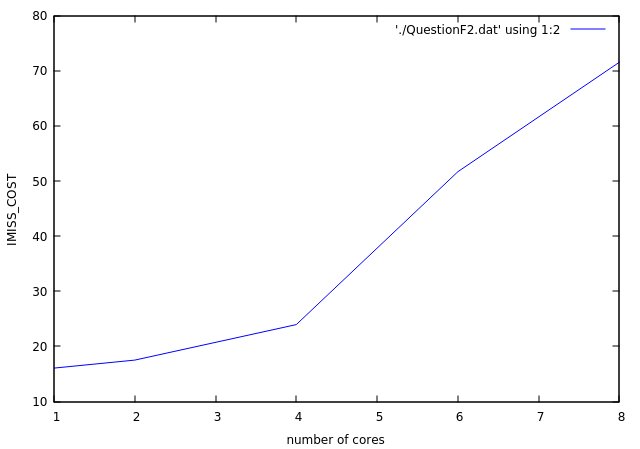
\includegraphics[width=8.5cm]{QuestionF2_1.png}
  \quad
  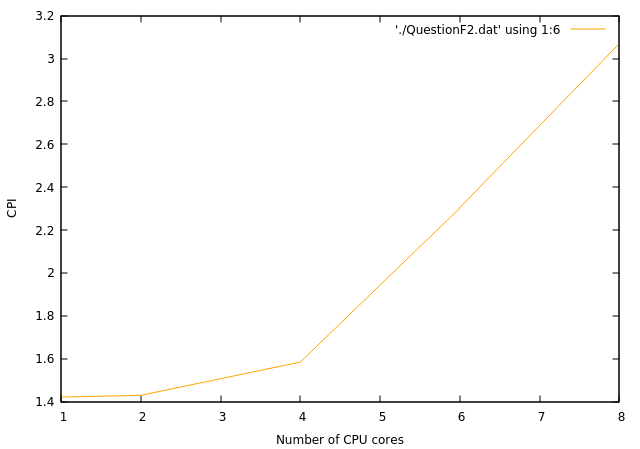
\includegraphics[width=8.5cm]{QuestionF2_5.png}
  \newline
  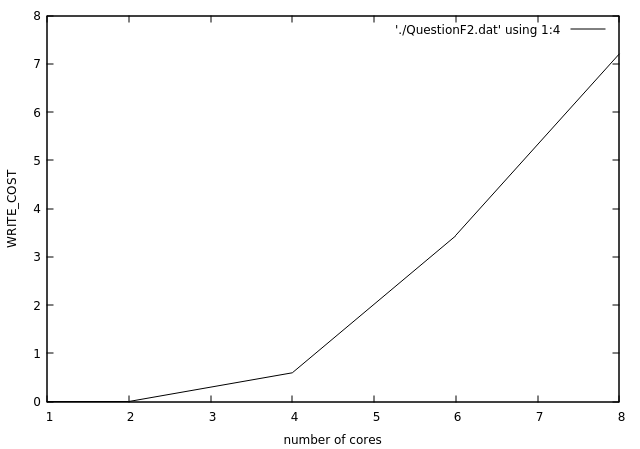
\includegraphics[width=8.5cm]{QuestionF2_3.png}
  \quad
  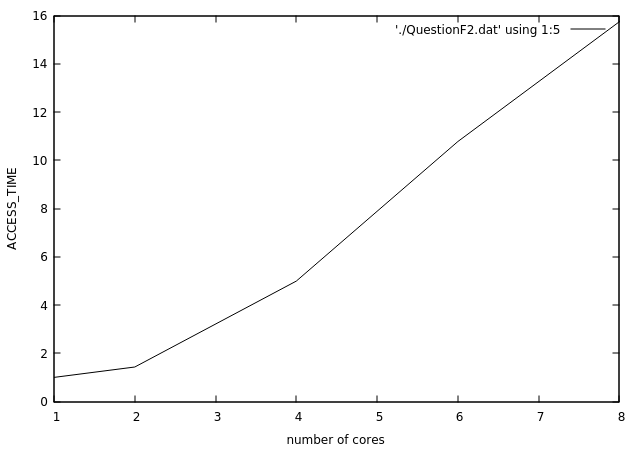
\includegraphics[width=8.5cm]{QuestionF2_4.png}
\end{center}

\subsection{Question F3}
La dégradation de la valeur du CPI est liée à l'augmentation du coût des MISS
mais également à l'augmentation du coût des écritures : en effet, parce que
les écritures sont prioritaires, les processeurs doivent supporter lors de leur
attente la congestion passive du bus ainsi qu'un supplément dû aux tampons
d'écritures postées.

\newpage

\subsection{Question G1}
\begin{center}
  \begin{tabular}{|c|c|c|c|}
    \hline
    \texttt{IMISS} & \texttt{DMISS} & \texttt{UNC} & \texttt{WRITE} \\ \hline
    $9$ & $9$ & $2$ & $2$ \\ \hline
  \end{tabular}
\end{center}

\subsection{Question G2}
Soit $F$ la fréquence, $n$ le nombre d'instructions de la transaction et $N$ le temps
total d'execution :
\begin{center}
  $F=\frac{n}{N}$\\
\end{center}
\begin{center}
  \begin{tabular}{|c|c|c|}
    \hline
     & Temps\_occupation & Fréquence \\ \hline
     \texttt{IMISS} & 9 & 0.006294\\ \hline
     \texttt{DMISS} & 9 & 0.006245\\ \hline
     \texttt{UNC  } & 2 & 0.000924\\ \hline
     \texttt{WRITE} & 2 & 0.100564\\ \hline
  \end{tabular}
\end{center}

\subsection{Question G3}
\begin{center}
  $BP=\sum Temps\_occupation \times F$
\end{center}
À partir de cette formule, on peut démontrer que la bande passante utilisée par
un processeur est $BP=0.315827$, soit $31.58\%$, théoriquement $3.1666$ coeurs
est la limite supportée par le PIBUS avant saturation.


\subsection{Bonus : \texttt{atomic\_increment}}
\lstinputlisting{atomic_increment.s}
\end{document}
